\documentclass[a4,center,fleqn]{NAR}

% Enter dates of publication
\copyrightyear{2008}
\pubdate{31 July 2009}
\pubyear{2009}
\jvolume{37}
\jissue{12}

\bibliography{paper-webserver.bib}

%\articlesubtype{This is the article type (optional)}

\begin{document}

\title{Spfy: distributed predictive genomics of E.coli with graph based result linkage}

\author{%
Corresponding Author\,$^{1,*}$,
First Co-Author\,$^{2}$
and Second Co-Author\,$^2$%
\footnote{To whom correspondence should be addressed.
Tel: +44 000 0000000; Fax: +44 000 0000000; Email: xxx@yyyy.ac.zz}}

\address{%
$^{1}$Affiliation of Corresponding Author
and
$^{2}$Affiliation of Both Co-Authors}
% Affiliation must include:
% Department name, institution name, full road and district address,
% state, Zip or postal code, country

\history{%
Received January 1, 2009;
Revised February 1, 2009;
Accepted March 1, 2009}

\maketitle

\begin{abstract}

\end{abstract}


\section{Introduction}
% new outline
% para
% 1. brief: WGS is standard
% 2. Big Problem: but tools are for individual analysis
% 3. 100,000 genomes, (lookup number for Enterobase, GenBank), how do we run analysis on it
% 4. previous methods (Galaxy/IRIDA: real-time, but no storage of results, other website examples - Denmark?), what problems they addressed
% 5. Problems that remain / lack of result storage means: recomputation, lost data, can't reference old analyses, not suited for "big data"
% 6. Solutions in general: store and increment, huga "big data" analyses, parallelization /queues
% para
% 1. Our specific problem, previous work
% 2. Why solving it is important (for Public health / research)
% 3. how we solved it
% para
% 4. benefits: rapid analyses in real-time -> huge comparisons, replace reference labs -> time & money saved, future work -> expand analyses, more genomes, more species
% 5. analyses modules -> conda -> IRIDA/Galaxy
% 6. short snippit on website link & github link

% 1. brief: WGS is standard
Whole genome sequencing (WGS) resolves the entire genetic content of an organism. WGS data can increase the resolution and sensitivity of bacterial surveillance \cite{ronholm2016navigating,lytsy2017time}, identification of potential disease mechanisms \cite{wang2014whole,yuen2015whole}, and clinical diagnoses \cite{willig2015whole,dewey2014clinical}.
% 2. Big Problem: but tools are for individual analysis
Targeted software, such as the Resistance Gene Identifier (RGI) \cite{mcarthur2013comprehensive} for antimicrobial resistance (AMR) gene prediction, Prokka for bacterial genome annotation \cite{doi:10.1093/bioinformatics/btu153}, and integrated platforms, such as the Bacterium Analysis Pipeline (BAP) \cite{thomsen2016bacterial} and the Integrated Rapid Infectious Disease Analysis (IRIDA) project \url{http://www.irida.ca/}, all leverage WGS data.
% 3. 100,000 genomes, (lookup number for Enterobase, GenBank), how do we run analysis on it
WGS generates data at a break-neck speed; for \textit{Escherichia coli} alone, the public genome databases EnteroBase \url{https://enterobase.warwick.ac.uk/} and GenBank \cite{doi:10.1093/nar/gks1195} have, respectively, 60,206 and 2,779,008 sequences uploaded.
To effectively exploit WGS "big-data" and maintain the rapid response time required by public health applications, one approach is to make results from WGS analysis integrated and progressive.
Typical bioinformatics software, such as RGI and Prokka, take single files as input, and integrated platforms, such as BAP and IRIDA, build workflows linking different analyses modules.
BAP and IRIDA begin to solve big-data challenges by offering a hosted solution which computes results in real-time, and distributes analyses across computing resources.
While effective for self-contained workflows, many comparative analyses such as predictive genomics methods would benefit from a broad WGS reference base.
To use vast amount of WGS data and maintain real-time results for comparative analyses, platforms would need store results in a way that avoids recomputation when adding new WGS data.
A resource framework in which WGS results are integrated and searchable; whereby the storage of results avoids recomputation, persists, and allows for iterative, on-going learning, will expand the capacity of current comparative bioinformatics analyses.
This increased capacity will further benefit surveillance, research, and clinical applications\par

% 1. Our specific problem, previous work
We have previously developed Superphy \cite{whiteside2016superphy}, an online predictive genomics platform targeting \textit{E. coli}.
Superphy integrates pre-computed results with domain-specific metadata to provide real-time analyses of epidemiology relations.
While this tool has been useful for the thousands of pre-computed genomes in its database, the current pace of genome sequencing requires real-time predictive genomic analyses of tens of thousands of genomes, and the long term storage and referencing of these results, something that the original SuperPhy platform was incapable of.
% 2. Why solving it is important (for Public health / research)
WGS offers improved resolution over traditional strain comparison methods, such as pulsed-field gel electrophoresis (PFGE) \cite{ronholm2016navigating}.
Though the cost of developing, approving, and transforming existing workflows from wet-lab to sequence prediction approaches is time consuming and expensive \cite{koser2012routine}, platforms can only perform real-time analyses and linkage to thousands of historical results by leveraging WGS.
% 3. how we solved it
In this study, we present an update to the SuperPhy platform, called Spfy.
The update rewrites result storage with backing by a graph database, takes a modular approach to tool integration, and distributes analyses over task queues, thereby allowing users to submit genomes and modules to run in parallel in real-time, and address code failures.
All results are stored as a series of linked nodes which enables the platform to build associations between results as they are generated. \par

% 4. benefits: rapid analyses in real-time -> huge comparisons, replace reference labs -> time & money saved, future work -> expand analyses, more genomes, more species
By integrating task distribution with graph storage, Spfy enables large-scale analyses, such as epidemiological associations between specific genotypes, biomarkers, host, source, and other metadata, and statistical significance testing of genome markers for user-defined groups.
Subtyping options are ..., pan-genome generation ..., group comparisons via Fisher's, ML, .... for E.coli.
By supporting multiple \textit{in-silico} subtyping options, the platform functions similar to a reference laboratory, with added support for big-data analyses.
Currently, the platform has been tested with XXX genome files and result storage for XX analyses modules.
Future work will focus on adding more analysis modules and supporting different species, which can be connected to the existing graph database without need for recalculation.
To complement existing platforms such as IRIDA, modules are self-contained and can easily be integrated into Galaxy \cite{goecks2010galaxy} based platforms.
The website and source code are available at \url{https://superphy.github.io/}. \par


% end of new intro

% **************************************************************
% Keep this command to avoid text of first page running into the
% first page footnotes
\enlargethispage{-65.1pt}
% **************************************************************

% Some general comments
% The NAR Database issue is more of a showcase then a rigorous exploration of software design choices.
% Given this focus, i would suggest the following:
% 1. Increase/highlight the discriptions of the functions and capabilities, maybe by adding a Functionality section
% 2. In the Implmentation (or Methods) section, only give a cursory description of the layout and components. Don't need to provide too much justification
% 3. Use the Results section to highlight the scope/size and speed. This can be short
% 4. In the Discussion, this is where i would expand on the justications and reasons for specific design choices. Pick 2-3 main ones and discuss those (i.e. don't need to justify our choice of documentation software). Also compare with other software in Discussion.
% 5. Add a conclusions section


\section{FUNCTIONALITY}
% ONLY FOCUS ON THE ANALYSIS MODULES
% Describe available functions in spfy
% para covering everything
Spfy performs reference laboratory tasks: O-antigen and H-antigen typing, Shiga-toxin (STX) typing,  virulence factor (VF) and antimicrobial resistance (AMR) gene determination, and related strain determination.
Spfy also performs bioinformatics analyses: pangenome generation, statistical significance testing of genome markers for user-defined groups, and AMR predictions using support vector machines (SVMs).

% para covering ectyper & RGI
To further characterize strains ... serotyping, which detects the presence of specific cell surface antigens.
O-antigen and H-antigen typing, and VF determination use our ECTyper \url{https://github.com/phac-nml/ecoli_serotyping} software.
ECTYper compares the user-submitted genomes against a curated set of sequences, an approach originally implemented in the VirulenceFinder \cite{joensen2014real} tool.
The Comprehensive Antibiotic Resistance Database (CARD) \cite{mcarthur2013comprehensive} maintains a set of known AMR genes and develops the Resistance Gene Identifier (RGI) program.
Both ECTyper and RGI are based off of BLAST \cite{pmid2231712}.

% para on phylotyper
Stx typing looks at ...
Phylotyper constructs phylogenetic trees and uses ancestral reconstruction to determine Stx-types ... others.
The software can also be used to generate trees and determine closely related strains.

% para on pangenome
Bacterial species, pan-genome ...Panseq \cite{laing2010pan}, Roary \cite{page2015roary}, chewBBACA \url{https://github.com/mickaelsilva/chewBBACA}, and Graphtyper \cite{Eggertsson148403} can compute these pan-genomic regions, and are freely available.
Spfy integrates panseq ...

% group comparisons
By retrieving results from the database, Spfy provides group comparisons using Fishers.
...

% Panpredic???

\section{IMPLEMENTATION}
% para: the semantic web
Spfy is built around semantic web technologies which focuses on describing the relaions between different datum \cite{berners2001semantic}.
In biological data, a semantic web focus describes individual data points by the type, for example as a genome, contiguous DNA sequence, or gene, and then link related data together in a queryable graph.
Semantic web technlogies allow new, not previously described data to be seemlessly incorporated to the existing graph, and has been proposed as a common standard for the open sharing of data \cite{horrocks2005semantic}.

% para: semantic web in spfy
In Spfy, the entirety of SuperPhy's previous code is replaced with methods for handling semantic web technologies.
Generalized functions are used to convert the results from different analysis modules into a graph object, and that graph object is used to update the main graph database; information contained in the WGS file is also converted into a graph object and stored.
The use of semantic web technologies allows results to be linked to the genomes they were computed from, and all data points to share a common datastructure that can be queried together.

% para: intro to the spfy stack
Spfy's server-side code is developed in Python and the website served to users is developed using the React JavaScript library.
When users upload genomes for analysis: (i) they first make the upload through the ReactJS-based website. 
The public web service accepts up to 200 MB of genome files (50 genomes compressed, or 120 genomes compressed).
(ii) When files are uploaded, the user-selected analysis options are enqueued into the Redis Queue \url{http://python-rq.org/} task queue.
Redis Queue consists of a Redis Database \url{https://redis.io/} and task queue workers which run as Python processes.
(iii) The workers dequeue the various analyses and run them in parallel and results are stored back in the Redis database.
(iv) Python functions are then used to parse the results and permanently store them in Blazegraph \url{https://www.blazegraph.com/} - a graph database.
The entire Spfy platform is packaged as a series of Docker \url{https://www.docker.com/} containers and orchestrated using Docker Compose \url{https://docs.docker.com/compose/}.

\subsection{Data Storage}
% para
% 0. Goals: big-data, everything linked, easy addition of new links
% 1. spfy is built around graph technologies
% 1. how we structure our graph
% 2. ontoogies used
% 3. inferencing
% 3 1/2. SPARQL queries
Graph databases focus on describing relationships between different data points, is one of the emerging \cite{de2015trends} database types used for biological data, and one of the core building blocks of a semantic web technology stack \cite{horrocks2005semantic}.
Spfy uses the RDFLib Python library \url{https://rdflib.readthedocs.org/} to represent all data meant for long-term storage.
When serotyping, VF, AMR predictions, and pangenome generation tasks are completed, the results are stored within the graph database.
% note: below is a feature in development
The permanent storage of results serve as a one-time cost, and allows population-wide analyses of all stored genomes; result storage also enables Spfy to avoid recomputation when the same analysis is re-run.

% para
% ontology
Ontologies are indices which define types of data and the relations between them.
By sharing ontologies, it is possible to link sources of data from different organizations together, and Spfy uses types defined in the  Genomic Epidemiology Application Ontology (GenEpiO) (\cite{griffiths2017context} and Feature Annotation Location Description Ontology (FALDO) \cite{bolleman2016faldo}.
Spfy also connects genomes, contiguous sequences (contigs), pangenome regions, and predicted genes and alleles in novel ways; to allow the presence of various genes to be infered from a genome description, realtionship links are generically named.
(see Figure \ref{fig-ontology})
Individual genes and pangenome regions are connected to all the contigs they are found on using this inferencing method, such that it is possible to determine all the genomes which contain a particular target sequence.

\begin{figure}[t]
\begin{center}
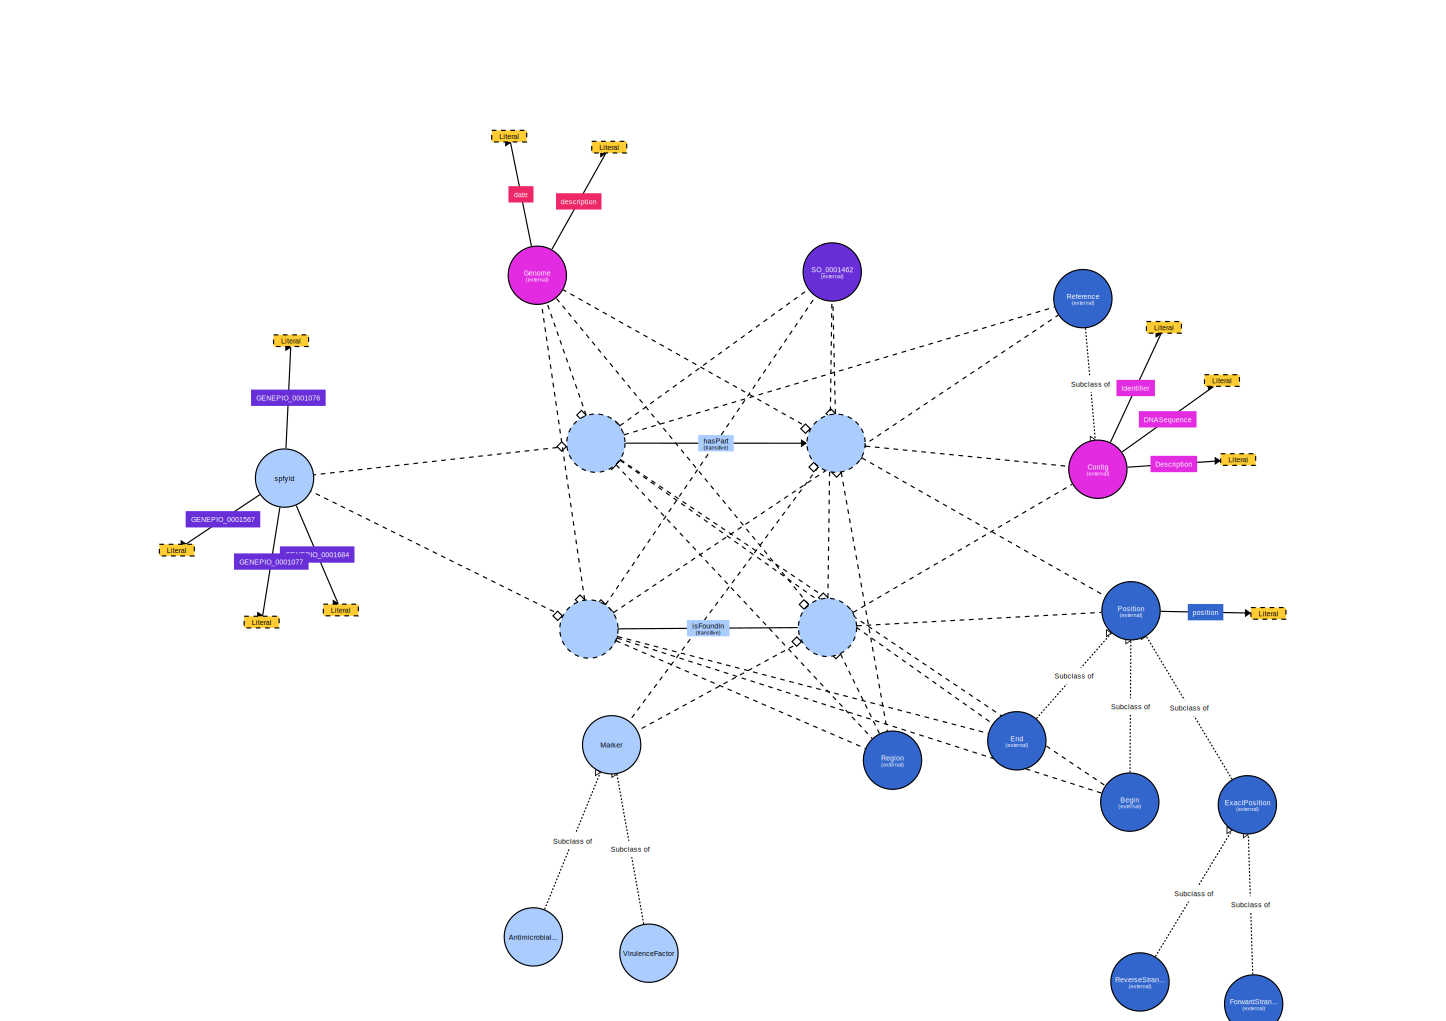
\includegraphics{images/spfy_ontology-1.svg}
\end{center}
\caption{Caption for figure within column.}
\label{fig-ontology}
\end{figure}

\subsection{Web design}
% para
% 1. goals: intuitive/familar, ease of use 
% 2. design specs
% 3. Google Material design
% 1. implementation: reactjs, react-md, ES6, JSX
% 4. separation from Flask layer

The front-end website displayed to users is written using the React JavaScript library \url{https://facebook.github.io/react/} as a single-page application to allow efficient data-flow without reloading the website.
To ensure a familiar user interface, we followed the Material Design specification \url{https://material.io/}, published by Google, and follow a card-based design.
(see Figure \ref{fig-results})
While data storage is graph-based, the results of various analysis modules are presented to users in a familiar tabular structure and available for download.
(see Figure \ref{fig-tables})

\begin{figure}[t]
\begin{center}
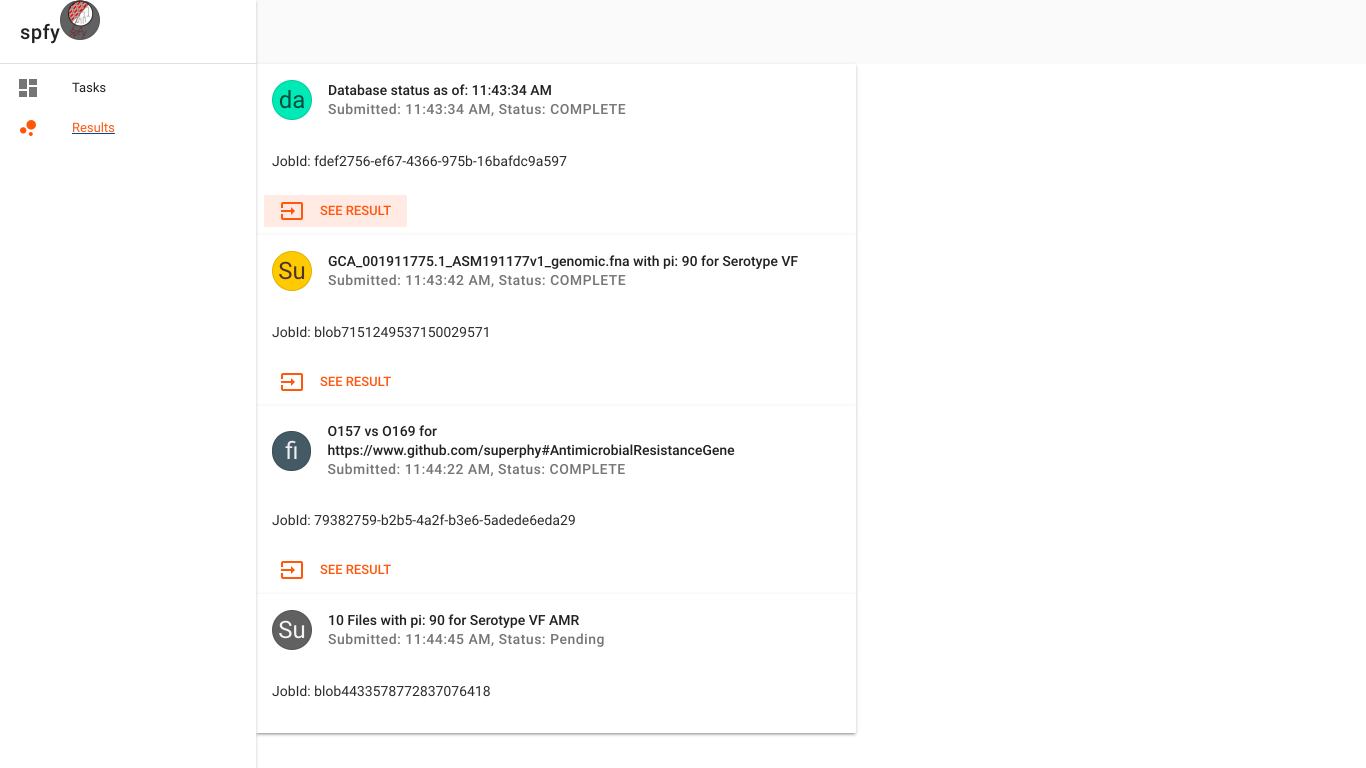
\includegraphics{images/results.png}
\end{center}
\caption{Caption for figure within column.}
\label{fig-results}
\end{figure}

\begin{figure}[t]
\begin{center}
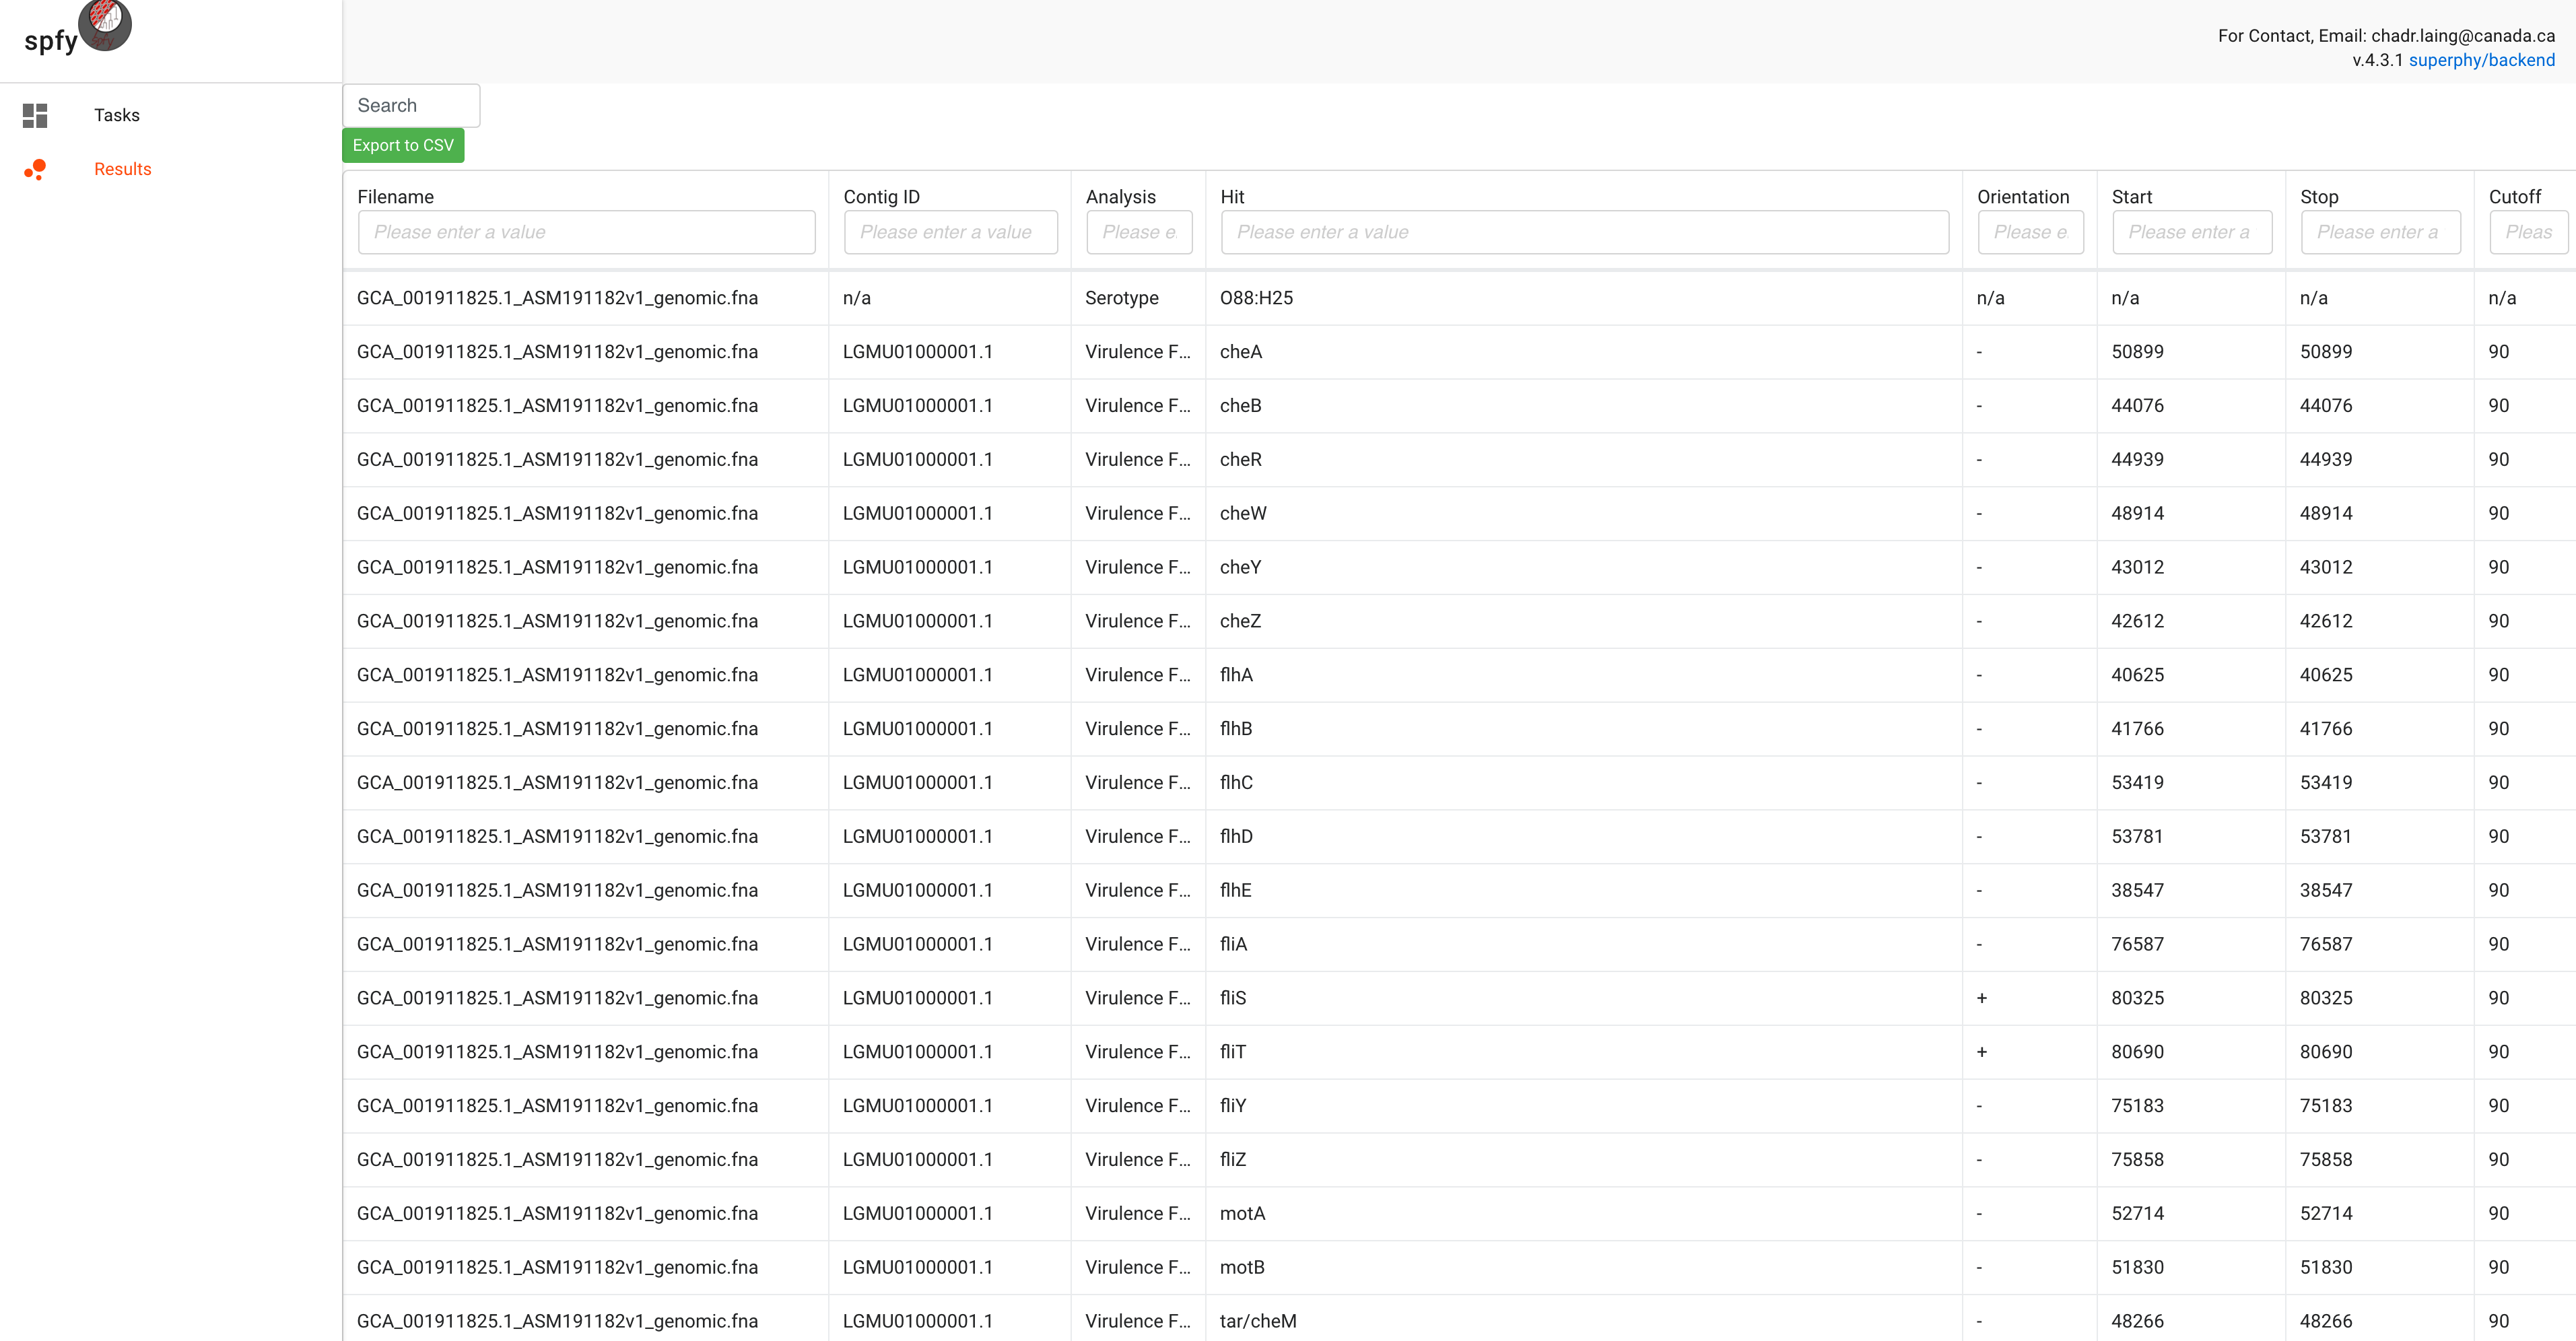
\includegraphics{images/tables.png}
\end{center}
\caption{Caption for figure within column.}
\label{fig-tables}
\end{figure}

\subsection{Real-time analysis pipelines}
% para
% 1. goals: real-time, support for pipelines (linked modules)
% 2. how pipelines have been handled in the past: Galaxy, other examples
% 3. Python, RQ
% para
% 1. how we implemented RQ
%	related: packaging of modules in conda

Task queues are processes which schedule code exection across available computing infrastructure.
In Spfy, the Python-based Redis Queue library \url{https://github.com/nvie/rq} is used to schedule analysis tasks and have them run asynchronously in response to user requests.
When a user submits files for analysis or population-wide anlayses, separate tasks are enqueued at different priorities, depending on when users might expect the result to be returned.
For example, population-wide analyses have a higher priority than bulk subtyping analyses, as we expect day-to-day web searches (for example, on Google) to respond instantly whereas a delay in subtyping is typical in similar web services such as the Center for Genomic Epidemiology Pipeline (CGE Pipeline) \cite{thomsen2016bacterial}.
Spfy enables processing of thousands of genome sequences by using task queue workers running in parallel, which also allows performance to scale to available infrastructure.
To ensure reliability of the platform, the open-source Sentry toolkit \url{https://github.com/getsentry/sentry} was integrated and used for real-time exception tracking.

% para
% 1. goals: scale analyses to "big-data", error handling
% 3. how we handle parallelization with RQ
% para
% 1. how many tasks have we tested this with
% 2. error handling: rq-dashboard, sentry
% 3. why options like sentry are better than traditional logging: scales well to tons (big-data levels) of tasks, groups the same errors together, reporting via email

% para
% 1. goals: why compartmentilizations
% 1. how we implemented docker
% 3. how this lets us replicate worker containers and link everything together

The Spfy platform depends on a series of webservers, databases, and task workers and uses \url{https://www.docker.com/}, a virtualization software package, to run self-contained operating systems on the same host computer.
Software packages are installed within the conatiners and the entire platform is networked together using Docker-Compose \url{https://docs.docker.com/compose/}.
(see Figure \ref{fig-docker})
Docker integration ensures that software dependencies, which typically must be manually installed \cite{doi:10.1093/bioinformatics/btu153,laing2010pan,inouye2014srst2,naccache2014cloud}, are handled automatically and that runtimes in one service are separated from another service.

\begin{figure}[t]
\begin{center}
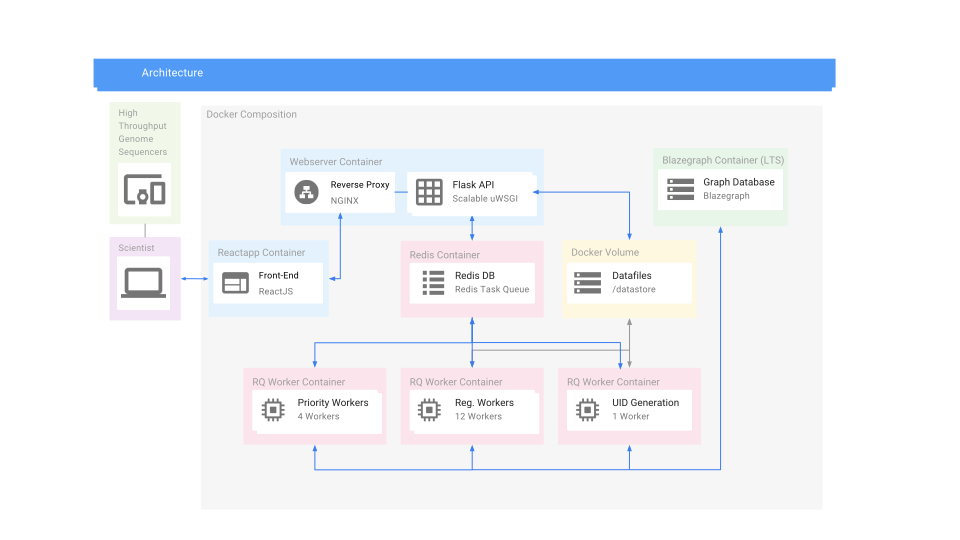
\includegraphics{images/docker.svg}
\end{center}
\caption{Caption for figure within column.}
\label{fig-docker}
\end{figure}

\subsection{Continuous integration and testing}
% Keep this short
% para
% 1. goals: why CI, testing is important
% 2. how we've implemented it, integration with github 

TravisCI \url{travisci.io}, a continuous integration (CI) platform, is integrated into Spfy's Github repository \url{https://github.com/superphy/backend} and runs tests ensuring functionality and backwards compatibility with any changes to the codebase.
The individual tests use PyTest \url{https://doc.pytest.org/} and are run within TravisCI's virtual environment.
The current build status can be checked either on our Gtihub repository or at \url{https://travis-ci.org/superphy/backend}.

\section{RESULTS}

% e.g.
% database statistics
We tested spfy with 55,353 samples genomes (267GB), storing both the entire genomes and results for all included analyses modules.
The resulting database had XYZ nodes and XYZ edges, with XYZ object properties.
This worked our to XYZ GB of data stored.

% analysis run-time / throughput with different levels of parallelization


\section{DISCUSSION}

% drawbacks - big data
Many previous bioinformatics software programs have been developed \textit{ad hoc}, without the use of software engineering principles \cite{de2015trends}.
Such tools were often script-based, with custom data formats, and only suitable for small collections of data \cite{de2015trends}.
While this was acceptable for smaller analyses, bioinformatic pipelines utilizing WGS data are larger and involve linked dependencies, which require the application of systems engineering principles \cite{schatz2015biological}.
Additionally, many subsets of biology now require the analyses of big-data, where the ability to perform computations in real-time, store data in flexible databases, and utilize a common application programming interface (API) linking resources are required \cite{swaminathan2016review}.

One of the key goals in developing Spfy is to maintain instantaneity: modern websites have accustomed users to instant results.
We attempt to use innovations in web development and bring a similar experience to Spfy as a predictive genomics platform for \textit{E. coli}.
% Mention where users / developers can find documentation
Spfy's main documentation and codebase are provided at \url{https://github.com/superphy/backend} and a developer guide is provided at \url{https://superphy.readthedocs.io/en/latest/}.

\subsection{Impact on Public Health Efforts}

% para
% focus on application
The isolation and characterization of bacterial pathogens are critical for Public Health laboratories to rapidly respond to outbreaks, and to effectively monitor known and emerging pathogens through surveillance programs.
Until recently, Public-health agencies relied on laboratory tests such as XYZ to characterize bacterial isolates in outbreak and surveillance settings.
The previous gold-standard in determining strain relatedness was pulsed-field gel electrophoresis (PFGE) {ronholm2016navigating}, which uses rare-cutting restriction enzymes to produce a unique banding pattern for each strain.
However, in \textit{Enterococcus faecium}, PFGE has been shown to misclassify 9 of 132 isolates, when compared to whole-genome sequencing (WGS) based discrimination \cite{pinholt2015multiple}.
In \textit{Klebsiella pneumoniae} \cite{marsh2015genomic}, \textit{Yersinia enterocolitica} \cite{gilpin2014limitations}, and \textit{Staphylococcus aureus} \cite{doi:10.1093/ofid/ofu096}, WGS was used to discriminate isolates after initial clustering by PFGE resulted in indistinguishable samples.
Examination of PFGE bands are also subjective, difficult to share \cite{lytsy2017time}, and collative platforms such as PulseNet reported \cite{gilpin2014limitations} that even after collecting 72\% of \textit{Campylobacter jejuni} in a given year in Minnesota (673 cases), 87\% of isolates could not be linked by PFGE pattern.
Antimicrobial resistance testing, virulence factor testing ...
However, current efforts are focused on predictive genomics, where the relevant phenotypic information can be determined through examination of the whole-genome sequence. 
, and as such can be used to evaluate the spread of outbreaks with better resolution and context than traditional methods \cite{ronholm2016navigating}.

% application: results similar to a wet-lab
Spfy uses WGS results.
After intial sequencing of new isolates, Spfy can be used in place of a traditional reference laborartory, to determine the O-type and H-type, Stx type, and all known VFs and AMR genes in real-time.
These results can be shared with other ageencies and researchers over the internet.
Futhermore, using Spfy's database of pre-processed genomes, Spfy can determine all strains a sample may be related to which is useful for ...
Cost benefits ...

\subsection{Comparison with other bioinformatic pipeline technologies}

% namely galaxy
Other scientific workflow technologies such as Galaxy \cite{goecks2010galaxy}, Kepler \cite{ludascher2006scientific}, and Taverna \cite{oinn2004taverna} have been applied to bioinformatic tasks.
Galaxy ...
Taverna ...
Kepler ...
To approach the challenge of integrating different bioinformatics programs, Spfy instead uses technologies prevalent in common web services not necessarily related to scientific workflows.
While we prefer to package individual bioinformatics programs using language-agnostic package managers such as Conda \url{https://conda.io/}, we do agree that suites of bioinformatics software benefit from having all dependencies installed and deployable in Docker containers \cite{di2015impact}.
These programs are connected to form a workflow using task queues; a design methodology used to offload long-running or non-instantaneous tasks over available computing infrastructure.
Unlike platforms such as Galaxy which favor a drag-and-drop design for building workflows, Spfy favors a tightly coupled approach explicitedy linking together different bioinformatics programs within the task queue implemntation.
In particular, Spfy uses asynchronous tasks queues which are tripped in response to user requests, thereby allowing immediate responsivity to users on the website, and processes generating human-readable results can be separated from processes handling long-term result storage.

% standard web tech means you can deploy to different cloud computing services
One of the key benefits of using more common-place technologies is the compatibility with other infrastructure resources.
Docker containerization is widely supported by cloud computing services: Amazon Web Services (AWS) \url{https://aws.amazon.com/docker/}, Google Cloud Platform (GCloud) \url{https://cloud.google.com/container-engine/}, and Microsoft Azure \url{https://azure.microsoft.com/en-us/services/container-service/}, and self-hosted cloud computing technologies such as OpenStack \url{https://wiki.openstack.org/wiki/Docker}.
% we may want to sign up for a free trial to give an example of this
Spfy packages compute nodes, which manage a collection of task queue workers, as reproducible Docker containers which can be networked together to form a compute cluster.
Docker containerization has a neglible impact on performance \cite{di2015impact}, and allows the platform to easily scale to demand.
In contrast to Galaxy, Spfy is a targeted approach building a predictive analytics platform for \textit{E. coli} which leverages generic web technologies to favor a responsive, big-data design strategy tackling the challenge \cite{fricke2014bacterial} of integrating results from multiple genomes and examining shared connections.
By packaging the individual bioinformatics software as Conda packages, they can be easily ported to Galaxy.

\subsection{Comparison with similar bioinformatic pipelines}

% para: \cite{naccache2014cloud}
% must install a ton of deps and even create dbs manually https://github.com/chiulab/surpi
% im not actually sure where they're getting the 'cloud-compatible' aspect of their paper from - its cloud compatible in that you deploy in the same manner as you would to bare-metal, but that's just like saying it 'runs on a computer'

% para: \cite{aanensen2016whole}
% makes some pretty pictures, but not really a pipeline

% para: \cite{joensen2014real,thomsen2016bacterial}
% we have a lot of similar directions to this, but just try to make it prettier, more friendly to use, and faster
The Bacterial Analysis Platform (BAP), developed out of the Technical University of Denmark, provides and integrated analysis pipeline for bacterial WGS data, as a web service.
BAP is novel in its combined approach to genome analysis as different programs, such as for VF and AMR determination, are included by default into the pipeline; Spfy provides similar functionallity with an expanded focus on integrated result storage and big-data analyses.
In place of a MySQL database for storing the location of result files, Spfy parses result data into graph objects and integrates results into a persistant graph database.
This enables Spfy to create large datasets where analysis results are linked to genomes, and to perform population-wide analyses.
On a per file basis, Spfy performs at a similar speed to BAP on predictive genomics tasks, though Spfy does not provide genome assembly services.
Spfy also processes XXXX files over XX tasks in XXXX time by using a novel approach of distributing computations over a task queue and multiple Docker compartmentalized containers.

\section{CONCLUSIONS}

\section{ACKNOWLEDGEMENTS}


\subsubsection{Conflict of interest statement.} None declared.
\newpage


\begin{thebibliography}{4}

% Format for article
\bibitem{1}
Author,A.B. and Author,C. (1992)
Article title.
\textit{Abbreviated Journal Name}, \textbf{5}, 300--330.

% Format for book
\bibitem{2}
Author,D., Author,E.F. and Author,G. (1995)
\textit{Book Title}.
Publisher Name, Publisher Address.

% Format for chapter in book
\bibitem{3}
Author,H. and Author,I. (2005)
Chapter title.
In
Editor,A. and Editor,B. (eds),
\textit{Book Title},
Publisher Name, Publisher Address,
pp.\ 60--80.

% Another article
\bibitem{4}
Author,Y. and Author,Z. (2002)
Article title.
\textit{Abbreviated Journal Name}, \textbf{53}, 500--520.

\end{thebibliography}

\end{document}
